\section{Improving Parameter Estimates by Solving Sequences of SIPs}\label{sec:mud-pde-sequence}
When progressing from two dimensions to five in the process of refining our estimate of $g$, we did so using an equal amount of parameter samples despite the volume of the spaces differing.
$\pspace$ increased by a factor of $64$ while all else was held constant.
Too many of the functions considered by the initial density were impractical to consider because of their roughness.
In the linear examples of \ref{subsec:linear_examples} it was shown that initial densities which ascribed higher likelihood to the true parameter led to MUD-point estimates that were more accurate.
By making better use of our model-evaluation budget of $1000$ samples for the PDE example, we find that both $\qoi_\text{1D}$ and $\qoi_\text{5D}$ perform significantly better in their ability to resolve $\paramref$.


%%%%%%%%%%%%%%%%%%%%%%%%%%%%%%%%%%%%%%%%%%%%%%%%%%%%%%%%%%%%%%%%
%%%%%%%%%%%%%%%%%%%%%%%%%%%%%%%%%%%%%%%%%%%%%%%%%%%%%%%%%%%%%%%%
\subsection{Motivations for a New Initial Density}
Reducing the volume of the support of the initial density will allow the samples drawn from it to better predict the collected data.
Recall from \ref{subsec:pde-example} that two maps were used to solve the SIP: $\qoi_{1D}$ and $\qoi_{2D}$ and MUD points were shown for representative examples.
We use the solutions from those examples\---namely the ratio which updates the initial density\---to inform the construction of a new initial density.
By considering the relationship between the parameters and the types of functions that could be possible given the solution to a 2-D inverse problem, we are able to create a more restricted parameter space in five dimensions.

For a detailed discussion of how a new initial density was constructed for this example, we refer the interested reader to Appendix~\ref{app:pde-5d-initial}.
We summarize the procedure briefly:
First we generate uniform i.i.d. samples in the three dimensions associated with the new knot points by defining independent bounds for each and taking samples from the cross-product of the directions.\footnote{
The bounds for each were determined by looking at piecewise-linear estimates of $g$ that come from sampling the updated density for the vector--valued solution.
}
We generate $\nsamps=1000$ i.i.d. samples from this 2-D uniform density
\footnote{
The (computational) cover is described by a procedure which involves the SVD of samples from the scalar--valued solutions in order to capture the correlation structure.
The use of the $\qoi_\text{1D}$ solution is due to the paucity of samples accepted from the vector--valued solution.
The structure of the latter updated density is more amenable to form a good estimate of this correlation direction in parameter space.
}
, and join them with the three other directions to form our new initial sample set, the functions from which generate the curves shown in Figure~\ref{fig:pde-highd-alt-initial-5d}.

\begin{figure}
\centering
  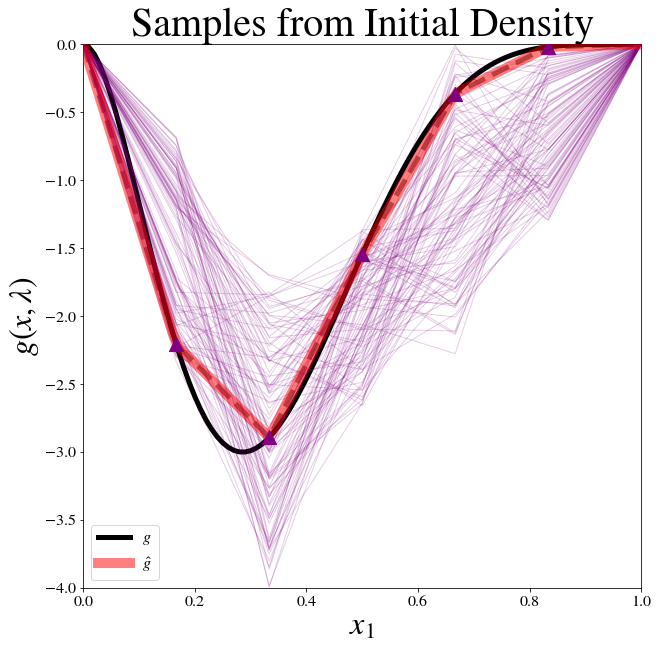
\includegraphics[width=0.675\linewidth]{figures/pde-highd/pde-highd_init_D5-alt}
\caption{
Initial density constructed for the second attempt at the five--dimensional inverse problem, with the structure of solutions learned from the 2-D example incorporated into the selection of bounds in each direction.
}
\label{fig:pde-highd-alt-initial-5d}
\end{figure}

The new initial curves in \ref{fig:pde-highd-alt-initial-5d}\---especially when contrasted to those in Fig.~\ref{fig:pde-highd-initial-5d}\---represent a far more reasonable set of possibilities.
The slope of the functions considered now all only have a single sign change, a marked improvement over the two or three that many samples from \ref{fig:pde-highd-initial-5d} exhibited.
We note that such considerations of smoothness could be avoided by parameterizing $g$ with a basis of some sort, but that problem is beyond the scope of this work.

%%%%%%%%%%%%%%%%%%%%%%%%%%%%%%%%%%%%%%%%%%%%%%%%%%%%%%%%%%%%%%%%
%%%%%%%%%%%%%%%%%%%%%%%%%%%%%%%%%%%%%%%%%%%%%%%%%%%%%%%%%%%%%%%%
\subsection{SIP Solutions using New Initial Density}
We now come to the solutions that arise from solving the same five--dimensional inverse problem of interpolating the values of $g$ through equispaced knot points, with both types of maps, in Figure~\ref{fig:pde-highd-5d-alt-mud}.
The difference in comparison to the solutions in Fig.~\ref{fig:pde-highd-5d-mud} is stark: no longer are the estimated functions dramatically under-estimating the local minimum of $g$.
To the extent to which they fail to adequately to do is due to the insufficient resolution of five knot points.

\begin{figure}
\centering
[TK - change figures to omit Q-Q, change savenames (pair = scalar|vector)]
  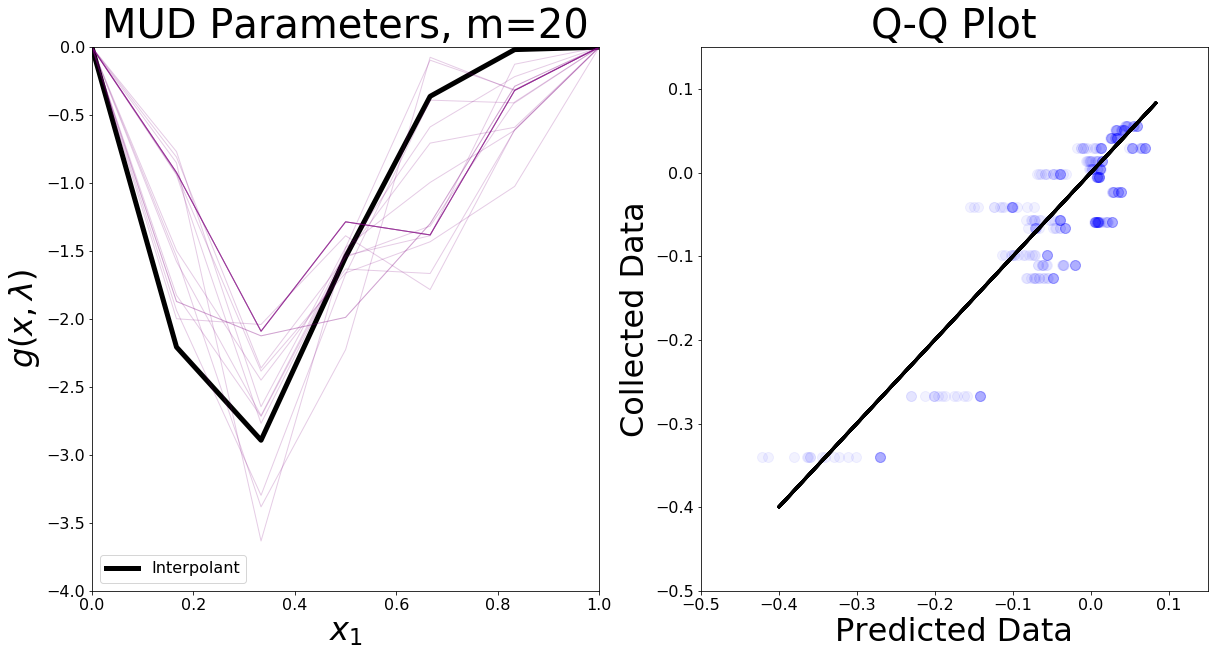
\includegraphics[width=0.95\linewidth]{figures/pde-highd/pde-highd_pair_D-alt-5-1_m20.png}
  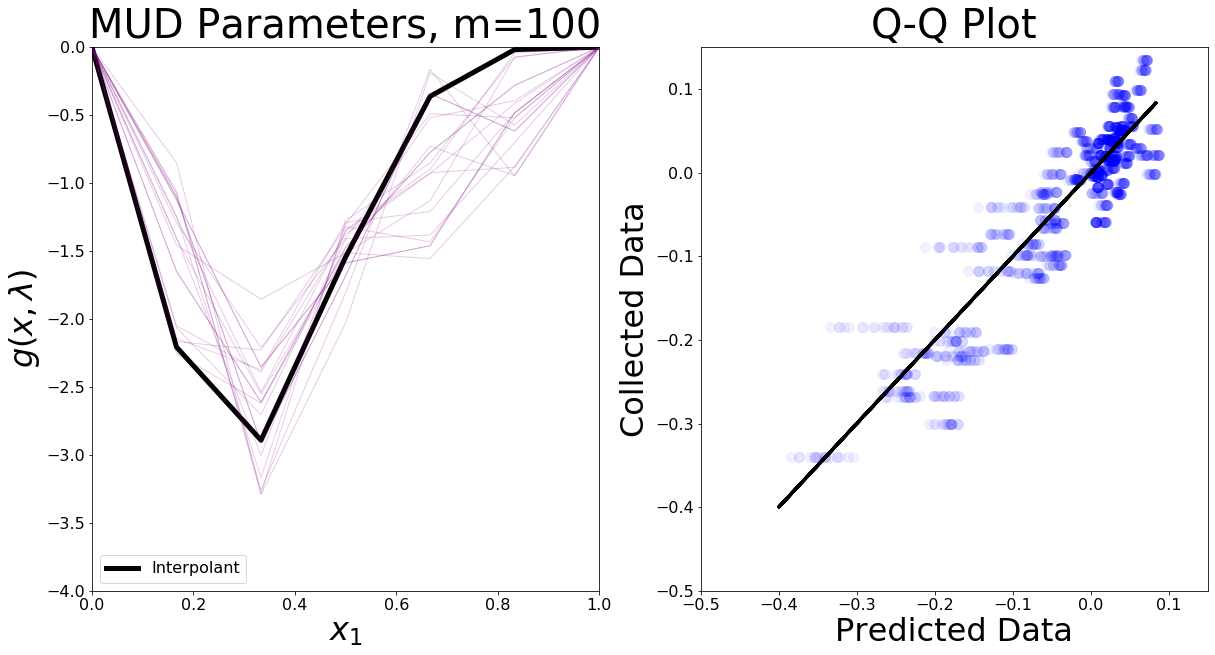
\includegraphics[width=0.95\linewidth]{figures/pde-highd/pde-highd_pair_D-alt-5-1_m100.png}
\caption{Solutions to the SIP using one hundred measurements.
(Top): Scalar-valued solutions for alternative approach to the five-dimensional problem.
(Bottom): Vector-valued solutions.
}
\label{fig:pde-highd-5d-alt-mud}
\end{figure}

Even when only twenty measurements are incorporated into constructing the QoI maps, there is a considerable improvement in the predicted boundary conditions when using a better initial density, as seen by comparing the solutions in \ref{fig:pde-highd-5d-alt-mud} to \ref{fig:pde-highd-5d-mud}.
Owing to the reduced volume of support for the initial density, both QoI maps resolve the residuals similarly, especially as more data is incorporated (shown in the bottom of \ref{fig:pde-highd-5d-alt-mud}).
Since ``unreasonable'' functions are no longer being considered, both maps produce qualitatively similar estimates.

\subsection{Demonstration of Reduction in Uncertainty}
As a final note on this experiment, we contrast the resulting $L^2$-errors to $g$ \footnote{derived from computational approximation with the trapezoidal rule} of these MUD solutions, to the previous two examples in Figure~\ref{fig:pde-highd-5d-hist}, to show a lineage of learning, so to speak.
With each successive problem, our uncertainty is reduced and our MUD solutions lower in variance and increase in accuracy.
Note that they appear to be moving towards a value away from zero, which represents a fixed bias (five equispaced knots can only approximate this $g$ so well).

\begin{figure}
\centering
  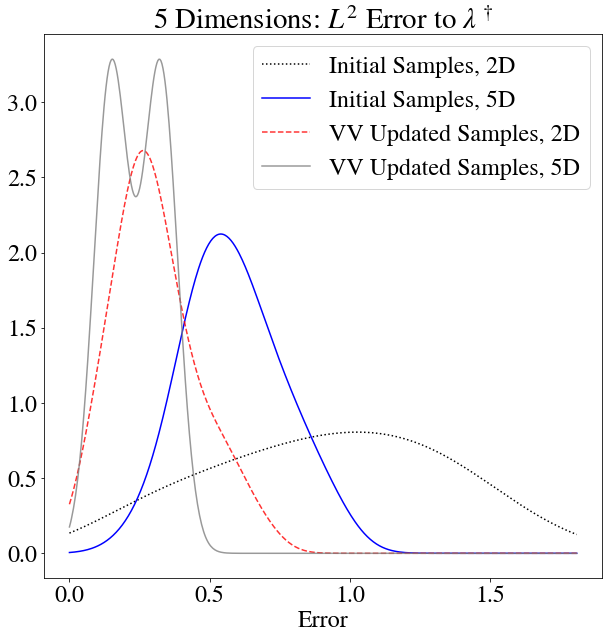
\includegraphics[width=0.675\linewidth]{figures/pde-highd/pde-highd_hist_D5_t5-0E-01}
\caption{
Comparison of the 2D initial errors to the 5D ones, as well as the reduction of uncertainty that solving a SIP problem for each provides.
}
\label{fig:pde-highd-5d-hist}
\end{figure}
